\chapter{Entwicklung des Testsystems}
\label{ch:model}

Um die in \cref{ch:caseStudy} beschriebene Fallstudie durchführen zu können, wurde zunächst TestingHadoop mithilfe des \gls{ss}"=Frameworks entwickelt.
Das Testsystem bildet \uA vereinfacht die für die Fallstudie relevanten YARN"=Komponenten ab und besteht aus den drei im Folgenden beschriebenen, architektonischen Schichten.

Da für die in \cite{Eberhardinger2018} durchgeführte Fallstudie das in diesem Kapitel beschriebene System genutzt wurde, wurden entsprechende Teile der Beiträge dieses Kapitels dort bereits publiziert.

\section{Grundlegende Architektur des Testmodells}
\label{sec:modelArchitecture}

Um Hadoop mit der Selfbalancing"=Komponente mit den in \cref{sec:requirements} beschriebenen Anforderungen prüfen zu können, wird mithilfe des \gls{ss}"=Frameworks ein vereinfachtes Modell der relevanten \gls{YARN}"=Komponenten entwickelt.
Dieses \gls{YARN}"=Modell wird mithilfe des Treibers mit dem realen Cluster verbunden, was durch hierfür entwickelte Scripte gesteuert wird.
Daraus resultiert folgende Drei"=Schichten"=Architektur für das gesamte Testmodell:

\begin{figure}[h]
    \includegraphics[width=0.6\columnwidth]{./resources/modelArchitecture.pdf}
    \caption{Grundlegende Architektur des Testmodells}
    \label{fig:modelArchitecture}
\end{figure}

Das \gls{YARN}"=Modell stellt die oberste Schicht des Testmodells dar.
Es bildet das Kernstück dieser Fallstudie, da dieses Modell mit den hierin abgebildeten \gls{YARN}"=Komponenten und Komponentenfehlern, dem Controller und dem Oracle direkt im Rahmen des modellbasierten Testens mit \gls{ss} interagiert.
Folgende Komponenten sind im \gls{YARN}"=Modell enthalten:

\begin{description}
    \item [Controller] \hfill \\
        Steuert den Ablauf einer Testausführung und das Zusammenspiel zwischen den Komponenten des \gls{YARN}"=Modells.
    \item [Relevante \gls{YARN}"=Komponenten und Eigenschaften] \hfill \\
        Bilden die grundlegende Architektur von Hadoop \gls{YARN} ab.
        Implementiert wurden in dieser Fallstudie die Nodes, Anwendungen, \glspl{Attempt} und \gls{Container} mit den jeweils relevanten Eigenschaften zur Durchführung der Fallstudie.
    \item [Komponentenfehler der \gls{YARN}"=Komponenten] \hfill \\
        Bilden die bei den \glspl{Test} zu injizierenden Komponentenfehler der jeweiligen \gls{YARN}"=Komponenten.
    \item [Oracle] \hfill \\
        Validiert die in Form von Constraints in den jeweiligen \gls{YARN}"=Komponenten implementierten Anforderungen.
    \item [Client] \hfill \\
        Dient zum starten und beenden von Benchmarks im Cluster.
    \item [Benchmark"=Controller] \hfill \\
        Enthält das Transitionssystem zur Auswahl der Benchmarks und steuert diese.
\end{description}

Die Verbindung zwischen dem \gls{YARN}"=Modell und dem realem Cluster bildet der Treiber.
Er besteht aus folgenden Komponenten:

\begin{description}
    \item [Parser] \hfill \\
        Verarbeitet die Monitoring"=Ausgaben vom realen Cluster und konvertiert diese für die Nutzung im \gls{YARN}"=Modell.
    \item [Connector] \hfill \\
        Abstrahiert die Verbindung zum realen Cluster und die dabei auszuführenden Befehle.
    \item [SSH"=Verbindung]  \hfill \\
        Stellt die Verbindung zum realen Cluster her.
\end{description}

Der Parser wird hierbei nur zur Durchführung des Monitoring benötigt und nutzt wiederum den Connector zum abrufen der Daten.
Andere Befehle und Zugriffe auf das reale Cluster, wie \zB das Injizieren von Komponentenfehlern, werden direkt mithilfe des Connectors durchgeführt.

In allen Komponenten des Modells werden zudem mithilfe des Frameworks log4net\footnote{\url{https://logging.apache.org/log4net/}}, Logausgaben durchgeführt.
Dies betrifft vor allem das Monitoring (vgl. \cref{subsec:yarnComponentInterface}), aber auch weitere Informationen wie zur Validierung der Constraints (vgl. \cref{subsec:oracleImpl}) oder reine Debug"=Informationen.
All diese Informationen werden im Programmlog zusammengefasst, welches auch zur Auswertung der ausgeführten \glspl{Test} dient.
Zu Analysezwecken im Fehlerfall wird zudem jede Kommunikation der SSH"=Verbindung in einem eigenen Log, dem SSH"=Log, abgespeichert (vgl. \cref{subsec:sshConnection}).

Die Implementierung des \gls{YARN}"=Modells wird in \cref{sec:yarnModel,sec:benchmarkController} beschrieben, die Implementierung des Treibers in \cref{sec:sshDriver}.
Die Umsetzung des realen Clusters wird in \cref{sec:realCluster} beschrieben.


\section{Implementierung des \acs{YARN}"=Modells}
\label{sec:yarnModel}

Das implementierte \ac{YARN}"=Modell besteht, wie bereits in \autoref{sec:modelArchitecture} gezeigt, aus fünf Komponenten und den Komponentenfehlern der hier relevanten \ac{YARN}"=Komponenten.
Die vier implementierten \ac{YARN}"=Komponenten sind die Anwendungen, ihre Attempts und Container, sowie die Nodes.
Zudem wurde eine Klasse implementiert, die zur Repräsentation des \ac{RM} dient, welche zudem auch als Controller im Rahmen des Testens mit \ac{ss} dient.
Einen Überblick über das Zusammenspiel des implementierten \ac{YARN}"=Modells gibt folgendes Klassendiagramm:

\begin{figure}[h]
    \includegraphics{./images/yarnModel_ls_MA.pdf}
    \caption[Grundlegender Aufbau des \acs{YARN}"=Modells]
        {Grundlegender Aufbau des \acs{YARN}"=Modells.
        Assoziationen und weitere Verbindungen zum Treiber und \acs{ss} sind hier aus Gründen der Übersichtlichkeit nicht dargestellt.}
    \label{fig:yarnModelClassDiagram}
\end{figure}

Im Folgenden werden zunächst die gemeinsam genutzten Bestandteile des \ac{YARN}"=Modells erläutert, welche nicht im Klassendiagramm enthalten sind, anschließend die fünf Komponenten des Modells, sowie die implementierten Komponentenfehler und basierend auf den in \autoref{sec:requirements} definierten Anforderungen implementierten Constraints.

\subsection{Gemeinsam genutzte Bestandteile des \acs{YARN}"=Modell}
\label{sec:yarnModelBasics}

\todo{Multihost-Mode irgendwo erklären}
\todo{irgendwo noch constraints einbauen}

\subsection{Relevante \acs{YARN}"=Komponenten}
\label{sec:yarnComponents}

\begin{figure}[h]
    \includegraphics[width=\columnwidth]{./images/yarnComponents.pdf}
    \caption[Für die Fallstudie relevante, implementierte \acs{YARN}"=Komponenten mit den wichtigsten Eigenschaften und Methoden]
        {Für die Fallstudie relevante, implementierte \acs{YARN}"=Komponenten mit den wichtigsten Eigenschaften und Methoden.
        Dies sind alle für die spätere Durchführung und zur Ausgabe des Zustandes (vgl. \autoref{sec:dataOrganisation}) wichtigen Eigenschaften und Methoden.
        Aus Gründen der Übersichtlichkeit sind die implementierten Komponentenfehler, einige der \texttt{IYarnReadable} bereitgestellten, relevanten Eigenschaften und Methoden, sowie die Klasse \texttt{YarnAppContainer} nicht aufgeführt.}
    \label{fig:yarnComponentsClassDiagram}
\end{figure}

\subsection{Implementierung des Clients}
\label{sec:yarnClient}

\subsection{Implementierung des Controllers}
\label{sec:yarnController}

\subsection{Implementierung des Oracles}
\label{sec:oracleImpl}

\todo{ab hier alte struktur!}

\begin{figure}
    \includegraphics[width=\columnwidth]{./images/yarnModel.png}
    \caption[Aufbau des YARN"=Modells]
    {Aufbau des YARN"=Modells.
        Das Modell wurde mithilfe des Klassendiagramm"=Designers in Visual Studio 2017 visualisiert.
        Daher werden Assoziationen mit höherer Multiplizität als 1, die daher mithilfe von \texttt{List<T>} umgesetzt wurden (\zB \texttt{YarnApp.Attempts}) im Diagramm nicht als Assoziationen zwischen den Klassen angezeigt.}
    \label{fig:yarnModel}
\end{figure}

\autoref{fig:yarnModel} beschreibt im Grunde bereits das gesamte von \sS verwendete YARN"=Modell.
Enthalten sind alle hier relevanten Komponenten sowie deren Eigenschaften.
Als Eigenschaften wurden die Daten aufgenommen, welche mithilfe von Shell"=Kommandos bzw. mithilfe der REST"=API von YARN ermittelt werden können.

\subsection{Modellierte YARN"=Komponenten}%\label{sec:yarnComponents}

Die abstrakte Basisklasse \texttt{YarnHost} stellt die Basis für alle Hosts des Clusters dar, also dem \texttt{YarnController} mit dem \ac{RM}, und dem \texttt{YarnNode}, was einen Node darstellt, auf dem die Anwendungen bzw. deren Container ausgeführt werden.
Die abstrakte Eigenschaft \texttt{YarnHost.HttpPort} dient als Hilfs"=Eigenschaft, da Controller und Nodes unterschiedliche Ports für die Weboberfläche nutzen, deren URL mit Port in der Eigenschaft \texttt{YarnHost.HttpUrl} abrufbar ist.
Sie wird daher vom Controller bzw. Node mit dem entsprechenden Port versehen.

Die mithilfe von \texttt{YarnApp} dargestellten Anwendungen werden mithilfe des \texttt{Bench"-Controller}s (vgl. \autoref{sec:appImplementation}) eines Clients (entsprechend repräsentiert durch die gleichnamige Klasse) gestartet.
Jeder Client kann nur eine Anwendung ausführen, daher gibt es die Möglichkeit, mehrere Clients zum Starten von mehreren gleichzeitig ausgeführten Anwendungen zu nutzen.
Die Anwendungen selbst enthalten neben grundlegenden Daten wie \zB den Namen auch einige Daten zum Ressourcenbedarf (Speicher und CPU).
Zwar gibt Hadoop nicht direkt die zu der Anwendung gehörigen Job"=Ausführungen an, allerdings können diese mithilfe der \texttt{YarnApp.AppId} sehr einfach ermittelt werden und dann in der Liste \texttt{YarnApp.Attempts} gespeichert werden.
Das Feld \texttt{YarnApp.IsKillable} gibt an, ob die Ausführung der Anwendung mit den aktuellen Daten im Modell durch den Komponentenfehler \texttt{YarnApp.KillApp} abgebrochen werden kann.
Abhängig ist das durch \texttt{YarnApp.FinalStatus}, was angibt, ob eine Anwendung erfolgreich oder nicht erfolgreich ausgeführt wurde oder die Ausführung noch nicht abgeschlossen ist (durch \texttt{EFinalStatus.UNDEFINED}).
Um die Komponentenfehler zu aktivieren bzw. bei Bedarf auch wieder zu deaktivieren, besitzen \texttt{YarnNode} und \texttt{YarnApp} jeweils die Eigenschaft \texttt{FaultConnector}, mit der auf den benötigten Connector zugegriffen werden kann.

Jede Ausführung \texttt{YarnAppAttempt} hat eine eigene ID und kann einer Anwendung zugeordnet werden.
Genau wie bei den Anwendungen selber wird hier direkt der Node gespeichert, auf welchem der \ac{AppMstr} ausgeführt wird und einen eigenen Container bildet, dessen ID direkt gespeichert wird.
Container (dargestellt durch \texttt{YarnAppContai"-ner}) existieren in Hadoop nur während der Laufzeit eines Programmes und enthalten nur wenige Daten, darunter ihr ausführender Node.
Jede Anwendung, deren Ausführungen und deren Container enthalten zudem den derzeitigen Status, ob die Komponente noch initialisiert wird, bereits ausgeführt wird oder beendet ist.
\texttt{EAppState.NotStartedYet} dient als Status, den es nur im Modell gibt und angibt, dass die Anwendung im späteren Verlauf der Testausführung gestartet wird.

Alle vier YARN"=Kernkomponenten implementieren das Interface \texttt{IYarnReadable}, was angibt, dass die Komponente ihren Status aus Hadoop ermitteln kann.
Entsprechend wird in allen Komponenten die Methode \texttt{ReadStatus()} implementiert, in welchem mithilfe des angegebenen Parsers auf den SSH"=Treiber zugegriffen werden kann und die Komponenten im Modell so ihre eigenen Daten aus dem realen Cluster ermitteln können.
Da die REST"=API ermöglicht, alle Daten auch über die reinen Listen zu erhalten anstatt ausschließlich über die Detailausgabe, besteht auch im Modell mithilfe der Eigenschaft \texttt{IsRequireDetailsParsing} das Ermitteln der Daten so einzustellen, dass die übergeordnete YARN"=Komponente bereits alle Daten ermittelt und der Untergeordneten zum Speichern (mittels \texttt{SetStatus()}) übergibt.
Als Basis dazu dient der \texttt{YarnController}, der dafür die Daten aller Anwendungen ausliest, die wiederum die Daten ihrer Ausführungen auslesen, welche dann die Daten ihrer Container auslesen und den Komponenten zum Speichern übergeben.

\subsection{Implementierung der Komponentenfehler}%\label{sec:implementedFaults}

Die Felder \texttt{YarnNode.NodeConnectionError} und \texttt{YarnNode.NodeDead} definieren die Komponentenfehler, wenn ein Node seine Netzwerkverbindung verliert bzw. beendet wird.
Die aus den Komponentenfehlern resultierenden Effekte werden in den dafür implementierten geschachtelten Klassen definiert.
\autoref{lst:faultInjection} zeigt beispielhaft die Implementierung und Injizierung des \texttt{NodeDead}"=Komponentenfehlers mithilfe des für den Node verwendeten \texttt{CmdConnector} (vgl. \autoref{sec:implementedConnectors}).
Die Injizierung des \texttt{NodeConnectionError}"=Komponentenfehlers und die Aufhebung beider Komponentenfehler sind analog implementiert.

\lstinputlisting[label=lst:faultInjection,
caption={[Injizierung eines Komponentenfehlers]
    Injizierung eines Komponentenfehlers (gekürzt).
    Sollte der Node nicht beendet werden, wird die Injizierung einmalig erneut versucht. \texttt{CmdConnector.Faulting} ist der für Komponentenfehler verwendete Connector.},
float,style=cs]
{./listings/faultInjectionExample.cs}

\subsection{Fehlerüberprüfung}%\label{sec:FaultTesting}

Um zu prüfen, ob sich das reale Cluster nach der Aktivierung bzw. Deaktivierung eines Komponentenfehlers korrekt rekonfiguriert, werden \emph{Constraints} genutzt.
\todo{Verweis zu Anforderungen}
Diese richten sich nach den funktionalen Anforderungen des Systems und prüfen, ob diese weiterhin eingehalten werden.
Da die funktionalen Anforderungen bei jeder YARN"=Komponente unterschiedlich sind, wurden diese mithilfe der Eigenschaft \texttt{IYarnReadable.Constraints} für jede Komponente einzeln definiert.
\autoref{lst:constraintDefinition} zeigt die Definition der Constraints für \texttt{YarnApp}, bei der die Anforderungen 1 und 3 eine Rolle spielen.
In jeder Komponente sind nur die funktionalen Anforderungen als Constraints implementiert, die für diese Komponente auch relevant sind.
Daher finden sich die beiden Anforderungen 2 und 4 nicht in der Klasse \texttt{YarnApp} wieder, letztere dafür aber \zB in \texttt{YarnNode}.

\lstinputlisting[label=lst:constraintDefinition,
caption={[Definition der Constraints in YarnApp]
    Definition der Constraints in \texttt{YarnApp}},
float,style=cs]
{./listings/constraints.cs}

Geprüft werden die Constraints im Anschluss an das Monitoring der einzelnen YARN"=Komponenten.
Wenn dabei die Bedingungen einer funktionalen Anforderungen nicht erfüllt werden, wird von den Constraints \texttt{false} zurückgegeben und so erkannt, dass bei dieser Komponente ein Fehler von Hadoop nicht selbst korrigiert wurde.
Die ID der Komponente wird daher entsprechend ausgegeben bzw. in der Logdatei gespeichert.
Zwar wäre es hier auch möglich gewesen, ähnlich wie in den Modellen der anderen Fallstudien, die mit dem \sS-Framework entwickelt wurden, eine Exception zu werfen, jedoch wurde hier darauf verzichtet, damit immer die Daten aller Komponenten geprüft werden können.
Dadurch kann erkannt werden, wenn mehrere Komponenten nicht den funktionalen Anforderungen entsprechen.

Nach der Überprüfung der Constraints wird abschließend geprüft, ob es dem Cluster möglich ist, sich überhaupt rekonfigurieren zu können.
Dies wird dadurch realisiert, dass geprüft wird, ob mindestens ein Node noch aktiv ist.
Dabei wird jedoch nicht der interne Fehlerstatus in \texttt{YarnNode.IsActive} oder \texttt{YarnNode.IsConnected} geprüft, sondern der beim Monitoring vom Cluster zurückgegebene \texttt{YarnNode.State}.
Nur wenn dieser den Wert \texttt{ENodeState.Running} hat, ist der Node aktiv und kann Anwendungen ausführen.
Das reale Hadoop"=Cluster kann sich somit nicht mehr rekonfigurieren und neue Container allokieren bzw. in der Ausführung befindliche Anwendungen und ihre Komponenten umverteilen, wenn kein Node den Wert \texttt{ENodeState.Running} hat.
\todo{Verweis auf Abschnitt, wo implementierung der Simulation genauer erklärt wird}
Kommt es zu diesem Fall, wird dies analog zu den Constraints ebenfalls ausgegeben und in der Logdatei vermerkt und die Ausführung des Simulationsschrittes fortgeführt, da die Daten aller Yarn"=Komponenten erst nach Abschluss der Simulation eines Schrittes ausgegeben werden.
Somit kann im Fehlerfall einfacher ermittelt werden, wie der Systemzustand zum Zeitpunkt des Fehlers war.


\section{SSH-Treiber}\label{sec:sshDriver}

Im Einführungstext zu diesem Kaptiel wurde bereits auf den grundlegenden Aufbau des Treibers eingegangen, der aus den drei einzelnen Komponenten Parser, Connector und der eigentlichen SSH-Verbindung besteht. Der Parser selbst besteht neben dem eigentlichen Parser zudem aus Datenhaltungs-Klassen für die relevanten YARN-Komponenten. Sie sind außerdem so aufgebaut, dass sie für beide hier implementierten Parser bzw. Connectoren für die Kommandozeilen-Befehle und die REST-API genutzt werden können.

\subsection{Integration im Modell}\label{sec:modelIntegration}

Hadoop besitzt zwei primäre Wege, um die Daten vom \ac{RM} bzw. dem \ac{TLS} ausgeben zu können. Dies ist zum einen die Kommandozeile, mithilfe der die Daten vom \ac{RM} und vom \ac{TLS} kombiniert ausgegeben werden, und die REST-API. Die benötigten Befehle für die Kommandozeile und deren Ausgaben sind in \autoref{app:hadoopCmds}, die für die REST-API benötigten URLs und deren Rückgaben in \autoref{app:hadoopRestApi} gelistet. Auf beiden Wegen können \uA die Daten zu folgenden Komponenten ausgegeben werden \cite{HadoopYarnTlServer271,HadoopYarnCmds271,HadoopRmApi271,HadoopNmApi271}:

\begin{description}
    \item[Anwendungen] als nach dem Status gefilterte Liste oder der Report einer Anwendung
    \item[Ausführungen] als Liste aller Ausführungen einer Anwendung oder der Report einer Ausführung
    \item[Container] als Liste aller Container einer Ausführung oder der Report eines Containers
    \item[Nodes] als Liste aller Nodes oder der Report eines Nodes
\end{description}

Zur Integration des Treibers wurden daher entsprechende Interfaces entwickelt, über die das Modell auf den eigentlichen Treiber zugreifen kann.

Die vier Interfaces \texttt{IApplicationResult}, \texttt{IAppAttemptResult}, \texttt{IContainerResult} und \texttt{INodeResult} dienen der Übergabe der geparsten Daten der einzelnen Komponenten an die korrespondierenden Komponenten im \sS-Modell. Sie enthalten jeweils alle relevanten Daten, die von Hadoop über die Kommandozeile oder die REST-API ausgegeben werden. Alle vier Interfaces implementieren zudem \texttt{IParsedComponent}, welches wiederum als Basis für die Übergabe der ausgelesenen Daten an \texttt{IYarnReadable.SetStatus()} im Modell dient.

Das Interface \texttt{IHadoopParser} dient als Einbindung des Parsers im Modell mithilfe von \texttt{IYarnReadable.Parser} und enthält für jede der acht relevanten Ausgaben von Hadoop entsprechende Methodendefinitionen.

Beim Interface \texttt{IHadoopConnector}, das im Modell den Connector über die \texttt{Fault"-Connector}-Eigenschaften von \texttt{YarnApp} und \texttt{YarnNode} einbindet, besitzt ebenfalls für jede der acht Datenrückgaben entsprechende Deklarationen, für Ausführungen und Container dabei jeweils vom \ac{RM} (\ac{NM} für Container) und vom \ac{TLS}. Auf die Nutzung des \ac{TLS} zum Ermitteln der Daten zu Anwendungen wird verzichtet. Dies liegt darin begründet, dass bei Nutzung der REST-API des \ac{RM} neben den vom \ac{TLS} bereitgestellten Daten einige weitere Informationen zu den Anwendungen ausgegeben werden \cite{HadoopRmApi271,HadoopYarnTlServer271}. Das Connector-Interface enthält darüber hinaus Deklarationen, um die im Modell implementierten Komponentenfehler im realen Cluster zu steuern und Anwendungen starten zu können. Architektonisch ist der Treiber zudem so aufgebaut, dass das Modell keine Kontrolle über den vom Parser benötigten Connector besitzt und die SSH-Verbindung ausschließlich vom Connector gesteuert werden kann.

\subsection{Implementierte Parser}\label{sec:implementedParsers}

Da die Daten für die relevanten Komponenten auf zwei Arten ermittelt werden können und unterschiedliche Ausgaben erzeugen, wurden auch für beide Arten ein Parser (\texttt{CmdParser} und \texttt{RestParser}) entwickelt. Da der Parser von außerhalb keinerlei weitere Informationen erhält außer der ID der zu parsenden YARN-Komponente, ist der Parser selbst dafür verantwortlich, die Daten von einem korrespondierenden Connector zu erhalten. Daher muss zur Initialisierung eines Parsers zunächst der korrespondierende Connector initialisiert werden. Da für die Nutzung der REST-API zum Teil die IDs der übergeordneten YARN-Komponenten ebenfalls nötig sind, ist der \texttt{RestParser} zudem auch dafür verantwortlich, die entsprechenden IDs zu ermitteln, bei der Nutzung der Kommandozeile reichen aufgrund der Befehlsstruktur die IDs der Komponenten selbst.

Die konkreten Implementierungen der auf \texttt{IParsedComponent} basierenden Übergabe"=Interfaces können ebenfalls als Bestandteil des Parsers angesehen werden. Sie wurden zudem so implementiert, dass sie für beide entwickelten Parser genutzt werden können.

Der grundlegende Ablauf ist bei jedem Parsing-Vorgang gleich. Zunächst werden, sofern benötigt, die benötigten YARN-Komponenten-IDs ermittelt und die Rohdaten mithilfe des Connectors von Hadoop abgefragt. Auch vom Parser wird dabei analog zum Modell das Abrufen der Daten ausschließlich mithilfe des Interfaces \texttt{IHadoopConnector} durchgeführt. Anschließend findet das eigentliche Parsing der Ausgabe von Hadoop statt, deren Daten direkt in der für die YARN-Komponente vorgesehene \texttt{IParsed"-Compo"-nent}-Implementierung gespeichert werden. Da Hadoop über die Kommandozeile die Daten in keinem standardisierten Format zurückgibt, wurde das Parsing der Rohdaten von Hadoop beim \texttt{CmdParser} in eigenem Code mithilfe von \emph{Regular Expressions} realisiert. Bei der Nutzung der REST-API werden die Daten dagegen im JSON-Format zurückgegeben \cite{HadoopYarnTlServer271,HadoopRmApi271,HadoopNmApi271}, wodurch diese mithilfe des \emph{Json.NET}-Frameworks\footnote{\url{https://www.newtonsoft.com/json}} deserialisiert und direkt als die entsprechende \texttt{IParsedComponent}-Implementierung gespeichert werden. Da \ac{RM} und \ac{TLS} verschiedene Daten einer YARN-Komponente ausgeben, werden, sofern nötig, \ac{RM} und \ac{TLS} abgefragt und die dabei ermittelten Daten zusammengeführt.

Eine erste Besonderheit bildet zudem das Abrufen und Parsen der Report-Daten mittels REST-API. Da die Listen hierbei als Array der einzelnen Reports zurückgegeben werden \cite{HadoopYarnTlServer271,HadoopRmApi271,HadoopNmApi271}, wird beim Parsen eines Ausführungs- oder Container-Reports die komplette Liste abgerufen und geparst. Anschließend wird in dieser Liste basierend auf der ID die benötigte Komponente herausgefiltert.

Die zweite Besonderheit bei der Nutzung der REST-API liegt darin, dass die Daten zu derzeit ausgeführten Container ausschließlich vom \ac{NM}, auf dem der Container ausgeführt wird, zurückgegeben werden können \cite{HadoopRmApi271,HadoopNmApi271}. Daher werden zur Ermittlung der Container-Listen alle Nodes abgefragt und anschließend die benötigten Container gefiltert.

Die geparsten Daten werden abschließend als das für die YARN-Komponente vorgesehene Interface zurückgegeben, was anschließend im Modell zum Speichern der Daten genutzt werden kann.

\subsection{Implementierte Connectoren}\label{sec:implementedConnectors}

Für die beiden Parser wurden die beiden korrespondieren Connectoren \texttt{CmdConnector} und \texttt{RestConnector} entwickelt. Während der Connector für die REST-API nur über eine SSH-Verbindung verfügt, besteht beim Connector für die Kommandozeile die Möglichkeit, mehrere einzelne SSH-Verbindungen zu nutzen. Dies ist damit begründet, dass zum Steuern der Komponentenfehler, was nur über die Kommandozeile möglich ist, eine eigene SSH-Verbindung genutzt wird. Zum Starten von Anwendungen besteht zudem die Möglichkeit, eine beliebige Anzahl an einzelnen SSH-Verbindungen aufzubauen, damit mehrere Anwendungen parallel gestartet werden können. Da die Daten der einzelnen YARN-Komponenten in der Fallstudie bevorzugt mithilfe der REST-API ermittelt werden, kann die dafür vorgesehene SSH-Verbindung des \texttt{CmdConnector} deaktiviert werden.

Da über die Kommandozeile die Befehle für die Daten vom \ac{TLS} die gleichen wie für die Daten vom \ac{RM} sind \cite{HadoopYarnTlServer271,HadoopYarnCmds271}, sind beim \texttt{CmdConnector} die \ac{TLS}-Methoden von geringer Bedeutung und nutzen daher ebenfalls die \ac{RM}-Methoden.

Der Connector ist beim Abrufen der Daten dafür zuständig, die dafür notwendigen Befehle auszuführen. Während dies für die Kommandozeilen-Befehle die entsprechenden Hadoop-Befehle sind, wird dies zum Abrufen der Daten über die REST-API mithilfe des Tools \emph{curl} durchgeführt. Die dabei zurückgegebenen Daten werden vom Connector ohne Verarbeitung zurückgegeben und können dann vom Parser verarbeitet werden.

Beim Steuern der Komponentenfehler wird vom Connector das für die Fallstudie entwickelte Start-Script verwendet. Nach dem eigentlichen Start bzw. Aufheben eines Komponentenfehlers wird vom Connector zudem überprüft, ob die Injizierung bzw. Aufhebung erfolgreich war. Während der Datenabruf sowie die Steuerung der Komponentenfehler synchron stattfindet, findet das Starten der Anwendungen asynchron und mithilfe des Benchmark-Scriptes statt. Da eine Ausführung einer YARN-Anwendung längere Zeit in Anspruch nehmen kann, wird dadurch die Ausführung von \sS nicht behindert und es können mehrere Anwendungen parallel ausgeführt werden.

\subsection{SSH-Verbindung}\label{sec:sshConnection}

Die SSH-Verbindung selbst ist der einzige Bestandteil des Treibers, welches kein entsprechendes Interface benötigt, die SSH-Verbindung wird ausschließlich vom Connector genutzt. Realisiert wird die Verbindung mithilfe des Frameworks SSH.NET,\footnote{\url{https://github.com/sshnet/SSH.NET}} weshalb die SSH-Verbindung im Treiber nur entsprechende Funktionen zum Aufbauen, Nutzen und Beenden der Verbindung enthält.

Um die Verbindung mit dem Cluster-PC aufzubauen, ist zudem ein dort installierter SSH-Key nötig. Ein Kommando auf dem Cluster-PC kann mithilfe der Treiberkomponente synchron und asynchron ausgeführt werden.

\section{Umsetzung des realen Clusters}
\label{sec:realCluster}

Da mithilfe der Plattform Hadoop"=Benchmark ein komplettes Hadoop"=Cluster auf einem PC ausgeführt werden kann und dieses speziell für die Forschung entwickelt wurde, wurde die Plattform für diese Fallstudie als Basis genutzt
Da Docker und Hadoop vor allem für den Einsatz in einer Linux"=Umgebung entwickelt wurden, werden für die Fallstudie zwei physische Hosts genutzt, auf denen das Cluster wahlweise auf einem oder auf beiden Hosts ausgeführt werden kann.
Zudem wird auf einem Host eine VM mit Windows 10 ausgeführt, das zum Ausführen des .NET"=Frameworks bzw. \ac{ss} benötigt wird.
Beide zum Einsatz kommenden Hosts sind jeweils mit einem Intel Core i5"=4570 @ 3,2 GHz x 4, 16 GB Arbeitsspeicher sowie einer SSD ausgestattet, auf der Ubuntu 16.04 LTS installiert ist.
Die Verbindung von Windows zu Linux auf beiden Hosts wird mithilfe von SSH"=Verbindungen umgesetzt.
Um den Ressourcenbedarf durch die von docker"=machine erzeugten VMs zu reduzieren, werden die Docker"=Container direkt auf den physischen Hosts ausgeführt:

\begin{figure}[h]
    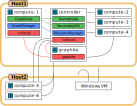
\includegraphics{./resources/caseStudyHadoopSetup.pdf}
    \caption[In der Fallstudie verwendetes Cluster"=Setup]
    {In der Fallstudie verwendetes Cluster"=Setup.
        Grün: \ac{HDFS}, Blau: YARN, Rot: Graphite.}
    \label{fig:caseStudyHadoopSetup}
\end{figure}

\todo{Irgendwo erwähnen, wie Docker-Container aufeinander aufbauen}
Durch die leicht veränderte Architektur stehen dem Cluster daher mehr Ressourcen zur Verfügung.
Zudem wird es mithilfe von von \emph{Docker Swarm} so ermöglicht, das Hadoop"=Cluster auf beiden Hosts auszuführen.
Neben der auf Host1 ausgeführten Basis des Clusters besteht die Möglichkeit, die auf Host2 ausgeführten Hadoop"=Nodes optional zum Cluster hinzuzufügen.
\todo{Basisanzahl Nodes erläutern}
Ein weiterer Unterschied zur originalen Plattform besteht darin, dass der Hadoop"=\ac{TLS} ebenfalls gestartet wird.
Zudem wurden einige Einstellungen von Hadoop so angepasst, dass defekte Nodes schneller erkannt werden.

Die Windows"=VM auf Host2 wird mithilfe von VirtualBox 5.2 ausgeführt.
Zum Abrufen von Daten mithilfe der REST"=API von Hadoop über die SSH"=Verbindungen wird \emph{curl}\footnote{\url{https://curl.haxx.se/}} 7.47 genutzt.
Zum Ausführen des Hadoop"=Clusters wird Docker in der Version 18.03 CE genutzt.

Um die in dieser Fallstudie benötigten Befehle einfach ausführen zu können, wurden zwei eigene Scripte erstellt, welche zum Teil auf den bestehenden Scripten der Plattform aufbauen.
Das Setup"=Script dient für folgende Zwecke:

\begin{itemize}
    \item Starten und Beenden des Clusters
    \item Starten und Beenden einzelner Hadoop"=Nodes
    \item Hinzufügen und Entfernen der Netzwerkverbindung des Docker"=Containers eines Hadoop"=Nodes
    \item Ausführen von eigenen Befehlen auf dem Docker"=Container des Hadoop"=Controllers
    \item Erstellen des Hadoop"=Docker"=Images
\end{itemize}

Das zweite erstellte Script dient ausschließlich zum Starten der Benchmarks.
Dazu werden die in der Plattform bereits enthaltenen Start"=Scripte aufgerufen, die für das konkrete Setup angepasst wurden.

